\documentclass[twoside]{book}

% Packages required by doxygen
\usepackage{fixltx2e}
\usepackage{calc}
\usepackage{doxygen}
\usepackage[export]{adjustbox} % also loads graphicx
\usepackage{graphicx}
\usepackage[utf8]{inputenc}
\usepackage{makeidx}
\usepackage{multicol}
\usepackage{multirow}
\PassOptionsToPackage{warn}{textcomp}
\usepackage{textcomp}
\usepackage[nointegrals]{wasysym}
\usepackage[table]{xcolor}

% Font selection
\usepackage[T1]{fontenc}
\usepackage[scaled=.90]{helvet}
\usepackage{courier}
\usepackage{amssymb}
\usepackage{sectsty}
\renewcommand{\familydefault}{\sfdefault}
\allsectionsfont{%
  \fontseries{bc}\selectfont%
  \color{darkgray}%
}
\renewcommand{\DoxyLabelFont}{%
  \fontseries{bc}\selectfont%
  \color{darkgray}%
}
\newcommand{\+}{\discretionary{\mbox{\scriptsize$\hookleftarrow$}}{}{}}

% Page & text layout
\usepackage{geometry}
\geometry{%
  a4paper,%
  top=2.5cm,%
  bottom=2.5cm,%
  left=2.5cm,%
  right=2.5cm%
}
\tolerance=750
\hfuzz=15pt
\hbadness=750
\setlength{\emergencystretch}{15pt}
\setlength{\parindent}{0cm}
\setlength{\parskip}{3ex plus 2ex minus 2ex}
\makeatletter
\renewcommand{\paragraph}{%
  \@startsection{paragraph}{4}{0ex}{-1.0ex}{1.0ex}{%
    \normalfont\normalsize\bfseries\SS@parafont%
  }%
}
\renewcommand{\subparagraph}{%
  \@startsection{subparagraph}{5}{0ex}{-1.0ex}{1.0ex}{%
    \normalfont\normalsize\bfseries\SS@subparafont%
  }%
}
\makeatother

% Headers & footers
\usepackage{fancyhdr}
\pagestyle{fancyplain}
\fancyhead[LE]{\fancyplain{}{\bfseries\thepage}}
\fancyhead[CE]{\fancyplain{}{}}
\fancyhead[RE]{\fancyplain{}{\bfseries\leftmark}}
\fancyhead[LO]{\fancyplain{}{\bfseries\rightmark}}
\fancyhead[CO]{\fancyplain{}{}}
\fancyhead[RO]{\fancyplain{}{\bfseries\thepage}}
\fancyfoot[LE]{\fancyplain{}{}}
\fancyfoot[CE]{\fancyplain{}{}}
\fancyfoot[RE]{\fancyplain{}{\bfseries\scriptsize Generated by Doxygen }}
\fancyfoot[LO]{\fancyplain{}{\bfseries\scriptsize Generated by Doxygen }}
\fancyfoot[CO]{\fancyplain{}{}}
\fancyfoot[RO]{\fancyplain{}{}}
\renewcommand{\footrulewidth}{0.4pt}
\renewcommand{\chaptermark}[1]{%
  \markboth{#1}{}%
}
\renewcommand{\sectionmark}[1]{%
  \markright{\thesection\ #1}%
}

% Indices & bibliography
\usepackage{natbib}
\usepackage[titles]{tocloft}
\setcounter{tocdepth}{3}
\setcounter{secnumdepth}{5}
\makeindex

% Hyperlinks (required, but should be loaded last)
\usepackage{ifpdf}
\ifpdf
  \usepackage[pdftex,pagebackref=true]{hyperref}
\else
  \usepackage[ps2pdf,pagebackref=true]{hyperref}
\fi
\hypersetup{%
  colorlinks=true,%
  linkcolor=blue,%
  citecolor=blue,%
  unicode%
}

% Custom commands
\newcommand{\clearemptydoublepage}{%
  \newpage{\pagestyle{empty}\cleardoublepage}%
}

\usepackage{caption}
\captionsetup{labelsep=space,justification=centering,font={bf},singlelinecheck=off,skip=4pt,position=top}

%===== C O N T E N T S =====

\begin{document}

% Titlepage & ToC
\hypersetup{pageanchor=false,
             bookmarksnumbered=true,
             pdfencoding=unicode
            }
\pagenumbering{roman}
\begin{titlepage}
\vspace*{7cm}
\begin{center}%
{\Large Erriez L\+CD Keypad Shield library for Arduino \\[1ex]\large 1.\+0.\+1 }\\
\vspace*{1cm}
{\large Generated by Doxygen 1.8.11}\\
\end{center}
\end{titlepage}
\clearemptydoublepage
\tableofcontents
\clearemptydoublepage
\pagenumbering{arabic}
\hypersetup{pageanchor=true}

%--- Begin generated contents ---
\chapter{L\+CD Keypad Shield library for Arduino}
\label{index}\hypertarget{index}{}\href{https://travis-ci.org/Erriez/ErriezLCDKeypadShield}{\tt }

This is a L\+CD Keypad Shield library for Arduino which supports the following features\+:


\begin{DoxyItemize}
\item 2x16 L\+CD using {\ttfamily Liquid\+Crystal.\+h}.
\item 5 pushbuttons connected to analog pin A0.
\item Button debouncing.
\item Backlight control (on/off).
\end{DoxyItemize}

\subsection*{Hardware}

Any Arduino board, tested on Arduino U\+NO.



\subsubsection*{Pins}

\tabulinesep=1mm
\begin{longtabu} spread 0pt [c]{*2{|X[-1]}|}
\hline
\rowcolor{\tableheadbgcolor}{\bf 2x16 L\+CD pins }&{\bf U\+N\+O/\+Leonardo/\+Mega2560  }\\\cline{1-2}
\endfirsthead
\hline
\endfoot
\hline
\rowcolor{\tableheadbgcolor}{\bf 2x16 L\+CD pins }&{\bf U\+N\+O/\+Leonardo/\+Mega2560  }\\\cline{1-2}
\endhead
RS &8 \\\cline{1-2}
EN &9 \\\cline{1-2}
D0 &4 \\\cline{1-2}
D1 &5 \\\cline{1-2}
D2 &6 \\\cline{1-2}
D3 &7 \\\cline{1-2}
Backlight &10 \\\cline{1-2}
\end{longtabu}
\subsection*{Example}

Arduion I\+DE $\vert$ Examples $\vert$ Erriez \hyperlink{class_l_c_d_keypad_shield}{L\+C\+D\+Keypad\+Shield}\+:


\begin{DoxyItemize}
\item \href{https://github.com/Erriez/ErriezLCDKeypadShield/blob/master/examples/LCDKeypadShield/LCDKeypadShield.ino}{\tt L\+C\+D\+Keypad\+Shield}
\end{DoxyItemize}

\subsection*{Documentation}


\begin{DoxyItemize}
\item \href{https://Erriez.github.io/ErriezLCDKeypadShield}{\tt Online H\+T\+ML}
\item \href{https://github.com/Erriez/ErriezLCDKeypadShield/raw/gh-pages/latex/ErriezLCDKeypadShield.pdf}{\tt Download P\+DF}
\end{DoxyItemize}

\subsection*{Usage}

{\bfseries Initialization}


\begin{DoxyCode}
1 \{c++\}
2 #include <ErriezLCDKeypadShield.h>
3 
4 LCDKeypadShield shield;
\end{DoxyCode}


\subsubsection*{Backlight control}

{\bfseries Backlight on}


\begin{DoxyCode}
1 \{c++\}
2 shield.backlightOn();
\end{DoxyCode}


{\bfseries Backlight off}


\begin{DoxyCode}
1 \{c++\}
2 shield.backlightOff();
\end{DoxyCode}


\subsubsection*{Display control}

All {\ttfamily L\+C\+D\+Keypad\+Shield.\+h} functions can be used.

{\bfseries Clear display}


\begin{DoxyCode}
1 \{c++\}
2 shield.clear();
\end{DoxyCode}


{\bfseries Set cursor}


\begin{DoxyCode}
1 \{c++\}
2 // First character first line
3 shield.setCursor(0, 0);
4 
5 // First character second line
6 shield.setCursor(0, 1);
7 
8 // Last character second line
9 shield.setCursor(15, 1);
\end{DoxyCode}


{\bfseries Print text}


\begin{DoxyCode}
1 \{c++\}
2 shield.print(F("Push the buttons"));
\end{DoxyCode}


\subsubsection*{Button control}

{\bfseries Get buttons}


\begin{DoxyCode}
1 \{c++\}
2 LCDButtons button = shield.getButtons();
3 // Returned button enum:
4 //   ButtonNone
5 //   ButtonRight
6 //   ButtonUp
7 //   ButtonDown
8 //   ButtonLeft
9 //   ButtonSelect
\end{DoxyCode}


\subsection*{Library dependencies}


\begin{DoxyItemize}
\item Arduino\textquotesingle{}s build-\/in {\ttfamily Liquid\+Crystal} library.
\end{DoxyItemize}

\subsection*{Library installation}

Please refer to the \href{https://github.com/Erriez/ErriezArduinoLibrariesAndSketches/wiki}{\tt Wiki} page.

\subsection*{Other Arduino Libraries and Sketches from Erriez}


\begin{DoxyItemize}
\item \href{https://github.com/Erriez/ErriezArduinoLibrariesAndSketches}{\tt Erriez Libraries and Sketches} 
\end{DoxyItemize}
\chapter{Hierarchical Index}
\section{Class Hierarchy}
This inheritance list is sorted roughly, but not completely, alphabetically\+:\begin{DoxyCompactList}
\item Liquid\+Crystal\begin{DoxyCompactList}
\item \contentsline{section}{L\+C\+D\+Keypad\+Shield}{\pageref{class_l_c_d_keypad_shield}}{}
\end{DoxyCompactList}
\end{DoxyCompactList}

\chapter{Class Index}
\section{Class List}
Here are the classes, structs, unions and interfaces with brief descriptions\+:\begin{DoxyCompactList}
\item\contentsline{section}{\hyperlink{class_l_c_d_keypad_shield}{L\+C\+D\+Keypad\+Shield} \\*L\+CD Keypad Shield class }{\pageref{class_l_c_d_keypad_shield}}{}
\end{DoxyCompactList}

\chapter{File Index}
\section{File List}
Here is a list of all documented files with brief descriptions\+:\begin{DoxyCompactList}
\item\contentsline{section}{\hyperlink{_l_c_d_keypad_shield_8cpp}{L\+C\+D\+Keypad\+Shield.\+cpp} \\*L\+CD Keypad Shield library for Arduino }{\pageref{_l_c_d_keypad_shield_8cpp}}{}
\item\contentsline{section}{\hyperlink{_l_c_d_keypad_shield_8h}{L\+C\+D\+Keypad\+Shield.\+h} \\*L\+CD Keypad Shield library for Arduino }{\pageref{_l_c_d_keypad_shield_8h}}{}
\end{DoxyCompactList}

\chapter{Class Documentation}
\hypertarget{class_l_c_d_keypad_shield}{}\section{L\+C\+D\+Keypad\+Shield Class Reference}
\label{class_l_c_d_keypad_shield}\index{L\+C\+D\+Keypad\+Shield@{L\+C\+D\+Keypad\+Shield}}


L\+CD Keypad Shield class.  




{\ttfamily \#include $<$Erriez\+L\+C\+D\+Keypad\+Shield.\+h$>$}

Inheritance diagram for L\+C\+D\+Keypad\+Shield\+:\begin{figure}[H]
\begin{center}
\leavevmode
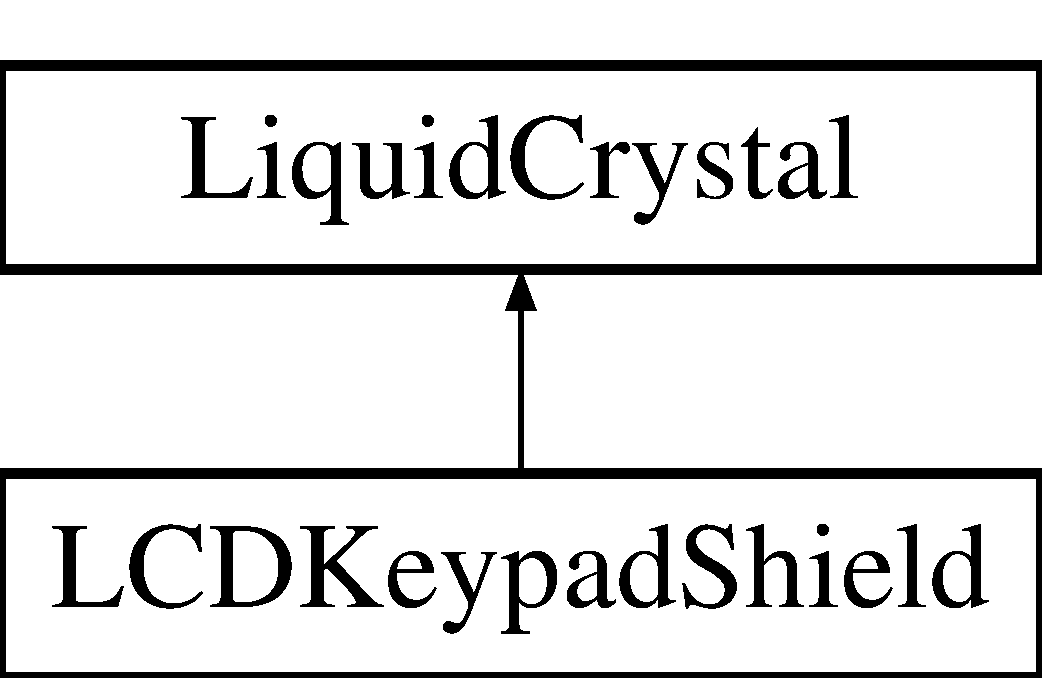
\includegraphics[height=2.000000cm]{class_l_c_d_keypad_shield}
\end{center}
\end{figure}
\subsection*{Public Member Functions}
\begin{DoxyCompactItemize}
\item 
\hyperlink{class_l_c_d_keypad_shield_ad26ce3a3a5c3300f0af024149bf87bb4}{L\+C\+D\+Keypad\+Shield} ()
\begin{DoxyCompactList}\small\item\em Constructor \hyperlink{class_l_c_d_keypad_shield}{L\+C\+D\+Keypad\+Shield} class. \end{DoxyCompactList}\item 
\hyperlink{_erriez_l_c_d_keypad_shield_8h_a024ede13291704606f2369e2d8798b1d}{L\+C\+D\+Button} \hyperlink{class_l_c_d_keypad_shield_ad8660e937c391344b3520d7610d7a3dc}{get\+Buttons} ()
\begin{DoxyCompactList}\small\item\em Read buttons from one analog pin. \end{DoxyCompactList}\item 
void \hyperlink{class_l_c_d_keypad_shield_abbdc6a191e247e5b8a12fe5d73b6431c}{backlight\+On} ()\hypertarget{class_l_c_d_keypad_shield_abbdc6a191e247e5b8a12fe5d73b6431c}{}\label{class_l_c_d_keypad_shield_abbdc6a191e247e5b8a12fe5d73b6431c}

\begin{DoxyCompactList}\small\item\em Turn backlight L\+ED on. \end{DoxyCompactList}\item 
void \hyperlink{class_l_c_d_keypad_shield_a7fcbbc1f3793be56707860e6892343fc}{backlight\+Off} ()\hypertarget{class_l_c_d_keypad_shield_a7fcbbc1f3793be56707860e6892343fc}{}\label{class_l_c_d_keypad_shield_a7fcbbc1f3793be56707860e6892343fc}

\begin{DoxyCompactList}\small\item\em Turn backlight L\+ED off. \end{DoxyCompactList}\end{DoxyCompactItemize}


\subsection{Detailed Description}
L\+CD Keypad Shield class. 

Definition at line 71 of file Erriez\+L\+C\+D\+Keypad\+Shield.\+h.



\subsection{Constructor \& Destructor Documentation}
\index{L\+C\+D\+Keypad\+Shield@{L\+C\+D\+Keypad\+Shield}!L\+C\+D\+Keypad\+Shield@{L\+C\+D\+Keypad\+Shield}}
\index{L\+C\+D\+Keypad\+Shield@{L\+C\+D\+Keypad\+Shield}!L\+C\+D\+Keypad\+Shield@{L\+C\+D\+Keypad\+Shield}}
\subsubsection[{\texorpdfstring{L\+C\+D\+Keypad\+Shield()}{LCDKeypadShield()}}]{\setlength{\rightskip}{0pt plus 5cm}L\+C\+D\+Keypad\+Shield\+::\+L\+C\+D\+Keypad\+Shield (
\begin{DoxyParamCaption}
{}
\end{DoxyParamCaption}
)}\hypertarget{class_l_c_d_keypad_shield_ad26ce3a3a5c3300f0af024149bf87bb4}{}\label{class_l_c_d_keypad_shield_ad26ce3a3a5c3300f0af024149bf87bb4}


Constructor \hyperlink{class_l_c_d_keypad_shield}{L\+C\+D\+Keypad\+Shield} class. 

This initializes the built-\/in Liquid\+Crystal library in 4-\/bit mode\+:
\begin{DoxyItemize}
\item RS, EN, D0, D1, D2 and D3 pins 
\end{DoxyItemize}

Definition at line 47 of file Erriez\+L\+C\+D\+Keypad\+Shield.\+cpp.



\subsection{Member Function Documentation}
\index{L\+C\+D\+Keypad\+Shield@{L\+C\+D\+Keypad\+Shield}!get\+Buttons@{get\+Buttons}}
\index{get\+Buttons@{get\+Buttons}!L\+C\+D\+Keypad\+Shield@{L\+C\+D\+Keypad\+Shield}}
\subsubsection[{\texorpdfstring{get\+Buttons()}{getButtons()}}]{\setlength{\rightskip}{0pt plus 5cm}{\bf L\+C\+D\+Button} L\+C\+D\+Keypad\+Shield\+::get\+Buttons (
\begin{DoxyParamCaption}
{}
\end{DoxyParamCaption}
)}\hypertarget{class_l_c_d_keypad_shield_ad8660e937c391344b3520d7610d7a3dc}{}\label{class_l_c_d_keypad_shield_ad8660e937c391344b3520d7610d7a3dc}


Read buttons from one analog pin. 

\begin{DoxyReturn}{Returns}
L\+C\+D\+Button enum 
\end{DoxyReturn}


Definition at line 66 of file Erriez\+L\+C\+D\+Keypad\+Shield.\+cpp.



The documentation for this class was generated from the following files\+:\begin{DoxyCompactItemize}
\item 
\hyperlink{_erriez_l_c_d_keypad_shield_8h}{Erriez\+L\+C\+D\+Keypad\+Shield.\+h}\item 
\hyperlink{_erriez_l_c_d_keypad_shield_8cpp}{Erriez\+L\+C\+D\+Keypad\+Shield.\+cpp}\end{DoxyCompactItemize}

\chapter{File Documentation}
\hypertarget{_l_c_d_keypad_shield_8cpp}{}\section{L\+C\+D\+Keypad\+Shield.\+cpp File Reference}
\label{_l_c_d_keypad_shield_8cpp}\index{L\+C\+D\+Keypad\+Shield.\+cpp@{L\+C\+D\+Keypad\+Shield.\+cpp}}


L\+CD Keypad Shield library for Arduino.  


{\ttfamily \#include $<$pgmspace.\+h$>$}\\*
{\ttfamily \#include \char`\"{}L\+C\+D\+Keypad\+Shield.\+h\char`\"{}}\\*


\subsection{Detailed Description}
L\+CD Keypad Shield library for Arduino. 

Source\+: \href{https://github.com/Erriez/ErriezLCDKeypadShield}{\tt https\+://github.\+com/\+Erriez/\+Erriez\+L\+C\+D\+Keypad\+Shield} Documentation\+: \href{https://erriez.github.io/ErriezLCDKeypadShield}{\tt https\+://erriez.\+github.\+io/\+Erriez\+L\+C\+D\+Keypad\+Shield} 
\hypertarget{_l_c_d_keypad_shield_8h}{}\section{L\+C\+D\+Keypad\+Shield.\+h File Reference}
\label{_l_c_d_keypad_shield_8h}\index{L\+C\+D\+Keypad\+Shield.\+h@{L\+C\+D\+Keypad\+Shield.\+h}}


L\+CD Keypad Shield library for Arduino.  


{\ttfamily \#include $<$Arduino.\+h$>$}\\*
{\ttfamily \#include $<$Liquid\+Crystal.\+h$>$}\\*
\subsection*{Classes}
\begin{DoxyCompactItemize}
\item 
class \hyperlink{class_l_c_d_keypad_shield}{L\+C\+D\+Keypad\+Shield}
\begin{DoxyCompactList}\small\item\em L\+CD Keypad Shield class. \end{DoxyCompactList}\end{DoxyCompactItemize}
\subsection*{Macros}
\begin{DoxyCompactItemize}
\item 
\#define \hyperlink{_l_c_d_keypad_shield_8h_a6ac777950db576df62346a5a7da5b3a7}{L\+C\+D\+\_\+\+P\+I\+N\+\_\+\+RS}~8\hypertarget{_l_c_d_keypad_shield_8h_a6ac777950db576df62346a5a7da5b3a7}{}\label{_l_c_d_keypad_shield_8h_a6ac777950db576df62346a5a7da5b3a7}

\begin{DoxyCompactList}\small\item\em L\+CD RS pin. \end{DoxyCompactList}\item 
\#define \hyperlink{_l_c_d_keypad_shield_8h_a2f5a69ed197584e7897bb7156a5e78fd}{L\+C\+D\+\_\+\+P\+I\+N\+\_\+\+EN}~9\hypertarget{_l_c_d_keypad_shield_8h_a2f5a69ed197584e7897bb7156a5e78fd}{}\label{_l_c_d_keypad_shield_8h_a2f5a69ed197584e7897bb7156a5e78fd}

\begin{DoxyCompactList}\small\item\em L\+CD EN pin. \end{DoxyCompactList}\item 
\#define \hyperlink{_l_c_d_keypad_shield_8h_a8a66f345a8eeae20b15759c685db6b57}{L\+C\+D\+\_\+\+P\+I\+N\+\_\+\+D0}~4\hypertarget{_l_c_d_keypad_shield_8h_a8a66f345a8eeae20b15759c685db6b57}{}\label{_l_c_d_keypad_shield_8h_a8a66f345a8eeae20b15759c685db6b57}

\begin{DoxyCompactList}\small\item\em L\+CD D0 pin. \end{DoxyCompactList}\item 
\#define \hyperlink{_l_c_d_keypad_shield_8h_ad6afc7eeae47046d74b841ad953a964a}{L\+C\+D\+\_\+\+P\+I\+N\+\_\+\+D1}~5\hypertarget{_l_c_d_keypad_shield_8h_ad6afc7eeae47046d74b841ad953a964a}{}\label{_l_c_d_keypad_shield_8h_ad6afc7eeae47046d74b841ad953a964a}

\begin{DoxyCompactList}\small\item\em L\+CD D1 pin. \end{DoxyCompactList}\item 
\#define \hyperlink{_l_c_d_keypad_shield_8h_aa160ab491002f5d4e9ca7dd586ecbae5}{L\+C\+D\+\_\+\+P\+I\+N\+\_\+\+D2}~6\hypertarget{_l_c_d_keypad_shield_8h_aa160ab491002f5d4e9ca7dd586ecbae5}{}\label{_l_c_d_keypad_shield_8h_aa160ab491002f5d4e9ca7dd586ecbae5}

\begin{DoxyCompactList}\small\item\em L\+CD D2 pin. \end{DoxyCompactList}\item 
\#define \hyperlink{_l_c_d_keypad_shield_8h_a67c78f256a4e1f357e9e1e7fbd65110c}{L\+C\+D\+\_\+\+P\+I\+N\+\_\+\+D3}~7\hypertarget{_l_c_d_keypad_shield_8h_a67c78f256a4e1f357e9e1e7fbd65110c}{}\label{_l_c_d_keypad_shield_8h_a67c78f256a4e1f357e9e1e7fbd65110c}

\begin{DoxyCompactList}\small\item\em L\+CD D3 pin. \end{DoxyCompactList}\item 
\#define \hyperlink{_l_c_d_keypad_shield_8h_a429569b08712c209a5799cf33e6153fa}{L\+C\+D\+\_\+\+B\+A\+C\+K\+\_\+\+L\+I\+G\+H\+T\+\_\+\+P\+IN}~10\hypertarget{_l_c_d_keypad_shield_8h_a429569b08712c209a5799cf33e6153fa}{}\label{_l_c_d_keypad_shield_8h_a429569b08712c209a5799cf33e6153fa}

\begin{DoxyCompactList}\small\item\em L\+CD backlight pin. \end{DoxyCompactList}\end{DoxyCompactItemize}
\subsection*{Enumerations}
\begin{DoxyCompactItemize}
\item 
enum \hyperlink{_l_c_d_keypad_shield_8h_a024ede13291704606f2369e2d8798b1d}{L\+C\+D\+Button} \{ \\*
{\bfseries Button\+None} = 0, 
{\bfseries Button\+Right} = 1, 
{\bfseries Button\+Up} = 2, 
{\bfseries Button\+Down} = 3, 
\\*
{\bfseries Button\+Left} = 4, 
{\bfseries Button\+Select} = 5
 \}\hypertarget{_l_c_d_keypad_shield_8h_a024ede13291704606f2369e2d8798b1d}{}\label{_l_c_d_keypad_shield_8h_a024ede13291704606f2369e2d8798b1d}
\begin{DoxyCompactList}\small\item\em L\+CD buttons. \end{DoxyCompactList}
\end{DoxyCompactItemize}


\subsection{Detailed Description}
L\+CD Keypad Shield library for Arduino. 

Source\+: \href{https://github.com/Erriez/ErriezLCDKeypadShield}{\tt https\+://github.\+com/\+Erriez/\+Erriez\+L\+C\+D\+Keypad\+Shield} Documentation\+: \href{https://erriez.github.io/ErriezLCDKeypadShield}{\tt https\+://erriez.\+github.\+io/\+Erriez\+L\+C\+D\+Keypad\+Shield} 
%--- End generated contents ---

% Index
\backmatter
\newpage
\phantomsection
\clearemptydoublepage
\addcontentsline{toc}{chapter}{Index}
\printindex

\end{document}
